\documentclass[10pt]{acmtrans2e}
\usepackage{hyperref}
\usepackage{amsmath}
\usepackage{amssymb}
\usepackage{amsfonts}
\usepackage{amscd}
\usepackage{amsmath}
\usepackage{latexsym}
\usepackage{graphicx}
\usepackage{geometry}
\usepackage{tikz-uml}
\usepackage{ifthen}
\usepackage{multicol}
\usepackage{paralist} % for compactitem und compactenum
% \usepackage{ellipsis}
\frenchspacing
\usepackage{nth}     % oridinal numbers: 1st, 2nd, ... by \nth{1}, \nth{2}, ...
                     % \usepackage[super]{nth} % Option 'super' not available at University
\usepackage{xspace}
\usepackage{enumitem}
\usepackage{listings}
\usepackage{epstopdf}

\hypersetup{
  colorlinks = false,
  urlcolor = blue,
  linkcolor = blue,
  pdfauthor = {Hao Lin},
  pdfkeywords = {Consensus clustering, $K$-means, utility function, MATLAB},
  pdftitle = {User Manual for KCC---a MATLAB package for K-means-based Consensus Clustering},
  pdfsubject = {KCC package},
  pdfpagemode = UseNone
}

\geometry{
  left=4cm,
  right=4cm,
  top=4cm,
  bottom=4cm
}

\newcommand{\Matlab}{\textsc{Matlab}}
\newcommand{\Octave}{\textsc{Octave}}
\newcommand{\KCC}{\textsf{KCC}\xspace} % package's name: \textsf{tboxIPscatt} and dynamic space

\newlength{\tabcont}
\newcommand{\tab}[1]{%
\settowidth{\tabcont}{#1}%
\ifthenelse{\lengthtest{\tabcont < 1cm}}%
{\makebox[1cm][l]{#1}\ignorespaces}%
{\makebox[2cm][l]{#1}\ignorespaces}%
}%

\newcommand{\syntax}[1]{\medskip
\noindent \textbf{Syntax:} \medskip

\texttt{#1}
}

\newenvironment{inputlist}
{\vspace*{0.25cm}
\noindent \textbf{Input parameters:}
\begin{itemize}
}  
{ 
\end{itemize}
}

\newenvironment{outputlist}
{\vspace*{0.075cm}
\noindent \textbf{Output parameters:}
\begin{itemize}
}  
{ 
\end{itemize}
}

\newenvironment{remark}
{\vspace*{0.1cm}
\noindent \textbf{Discussion:} \medskip

}
{
\vspace*{0.2cm}
}

\newenvironment{example}
{\vspace*{0.1cm}
\noindent \textbf{Example:} \vspace*{0.15cm}

\setlength{\parskip}{0.5ex plus 0.5exminus 0.2 ex}
}
{\medskip
}

\newcommand{\paramitem}[2]{\item[] \tab{\texttt{#1}} \tab{: #2} }

\firstfoot{}
\runningfoot{}

\markboth{Hao Lin}{User Manual for \KCC---a {MATLAB} package for K-means-based Consensus Clustering}

\title{User Manual for \KCC---a {MATLAB} package for K-means-based Consensus Clustering} 

% \author{Hao Lin}
% \orcid{0000-0002-1921-3036}
% \email{linh@in.tum.de}
% \affiliation{%
%   \institution{Department of Informatics, Technical University of Munich}
%   \streetaddress{Boltzmannstr. 3}
%   \city{Garching}
%   \postcode{85748}
%   \country{Germany}
% }

% \author{Hongfu Liu}
% \email{hongfuliu@brandeis.edu}
% \affiliation{%
%   \institution{Michtom School of Computer Science, Brandeis University}
%   \streetaddress{415 South St}
%   \city{Waltham}
%   \state{MA}
%   \postcode{02453}
%   \country{USA}
% }

% \author{Junjie Wu}
% \authornote{Corresponding Author}
% \email{wujj@buaa.edu.cn}
% \affiliation{%
%   \institution{School of Economics and Management, Beihang University}
%   \streetaddress{37 Xueyuan Rd}
%   \city{Haidian District}
%   \state{Beijing}
%   \postcode{100191}
%   \country{China}
% }

% \author{Hong Li}
% \email{hong_lee@buaa.edu.cn}
% \affiliation{%
%   \institution{School of Economics and Management, Beihang University}
%   \streetaddress{37 Xueyuan Rd}
%   \city{Haidian District}
%   \state{Beijing}
%   \postcode{100191}
%   \country{China}
% }

% \author{Stephan Günnemann}
% \email{guennemann@in.tum.de}
% \affiliation{%
%   \institution{Department of Informatics, Technical University of Munich}
%   \streetaddress{Boltzmannstr. 3}
%   \city{Garching}
%   \postcode{85748}
%   \country{Germany}
% }

\author{
Hao Lin\footnote{Department of Informatics, Technical University of Munich, Germany,
\textsf{\href{mailto:linh@in.tum.de}{linh@in.tum.de}}.}, \quad
Hongfu Liu\footnote{Michtom School of Computer Science, Brandeis University, USA, \textsf{\href{mailto:hongfuliu@brandeis.edu}{hongfuliu@brandeis.edu}}.}, \quad
Junjie Wu\footnote{School of Economics and Management, Beihang University, China, \textsf{\href{mailto:wujj@buaa.edu.cn}{wujj@buaa.edu.cn}}.}, \quad
Hong Li\footnote{School of Economics and Management, Beihang University, China, \textsf{\href{mailto:hong_lee@buaa.edu.cn}{hong\_lee@buaa.edu.cn}}.}, \quad
Stephan Günnemann\footnote{Department of Informatics, Technical University of Munich, Germany, \textsf{\href{mailto:guennemann@in.tum.de}{guennemann@in.tum.de}}.}
}
\date{User Manual for \KCC, updated \today}

\begin{document}

\maketitle

\vspace*{-0.5cm}

\section{Introduction}

This user manual systematically presents the usage of the \Matlab{} package on K-means-based Consensus Clustering (KCC) accompanying the following paper:
\begin{center}
\begin{minipage}{0.90\textwidth}
Hao Lin, Hongfu Liu, Junjie Wu, Hong Li, and Stephan Günnemann. 2022. Algorithm xxxx: KCC: A MATLAB Package for K-means-based Consensus Clustering. \emph{ACM Trans. Math. Softw}.
\end{minipage}
\end{center}

\noindent The package was developed and tested in \Matlab{} R2012a under Linux. {\color{red}To those without access to \Matlab{} and those who prefer to use free open source software, we also investigate the usage of \KCC with \Octave{}, and find it is also compatible with \Octave{} without additional efforts. \Octave{} version?}. 

For package installation, you need to first unpack the compressed archive into your current directory. It consists of a \emph{source code} folder \textsf{Matlab}, a folder \textsf{userManual} with this comprehensive \emph{user manual}, and a \emph{license} file \textsf{LICENSE} indicating that the package is distributed under GNU GENERAL PUBLIC LICENSE (Version 3). Then under the \textsf{Matlab} folder, you need to add one of its subfolder, i.e., the \textsf{Src} folder, to the \Matlab{} path. The directory structure of the \textsf{Matlab} folder is described as follows.
% All computations in this \emph{user guide} were carried out on a workstation with an Intel(R) Core(TM) i7-3770 CPU with 3.40\,GHz and 32\,GByte RAM. For the given code snippets we recommend more than 5\,GByte RAM. This, in particular, is true for the three-dimensional reconstruction example as it is the most RAM-consuming one.
% It can be downloaded from the ACM Collected Algorithms (CALGO). 

% \setlength{\columnseprule}{0.25pt}
% \setlength{\columnsep}{10pt}
% \begin{multicols}{2}[][10mm]
\begin{compactitem}
  \item \textsf{Src} (core functions for conducting KCC)
  \begin{compactitem}
   \item \textsf{BasicCluster\_RFS.m} (function to generate BPs with RFS)
   \item \textsf{BasicCluster\_RPS.m} (function to generate BPs with RPS)
   \item \textsf{Preprocess.m} (function to prepare for consensus clustering)
   \item \textsf{KCC.m} (consensus function)
   \item \textsf{exMeasure.m} (function to compute validity scores for clustering results)

   \item \textsf{load\_sparse.m} (auxiliary function to load input text data as a sparse matrix)
   \item \textsf{hungarian.m} (auxiliary function for cluster label assignment)
   \item \textsf{BasicCluster\_RPS\_missing.m} (auxiliary function to generate IBPs with strategy-I)
   \item \textsf{addmissing.m} (auxiliary function to generate IBPs using strategy-II)
   \item \textsf{distance\_*} (distance functions)
   \item \textsf{gClusterDistribution.m} (auxiliary function to calculate cluster distribution for BPs)
   \item \textsf{Ucompute.m, Ucompute\_miss.m} (auxiliary function for utility calculation)
   \item \textsf{gCentroid.m, gCentroid\_miss.m} (auxiliary function for centroid update)
   \item \textsf{sCentroid.m, sCentroid\_miss.m} (auxiliary function for centroid initialization)
  \end{compactitem}
  \item \textsf{Drivers} (illustrative examples)
  \begin{compactitem}
   \item \textsf{data} (input data for illustration)
   \item \textsf{demo.m} (function for KCC with different utility functions)
   \item \textsf{demoIBPI.m} (function for KCC with IBPs generated by strategy-I)
   \item \textsf{demoIBPII.m} (function for KCC with IBPs generated by strategy-II)
   \item \textsf{demoNumberBP.m} (function for KCC with varying number of BPs)
   \item \textsf{demoStrategyBP.m} (function for KCC with RFS strategy for BP generation)
  \end{compactitem}
\end{compactitem}
% \end{multicols}

\begin{figure*}[!bt]
\centering
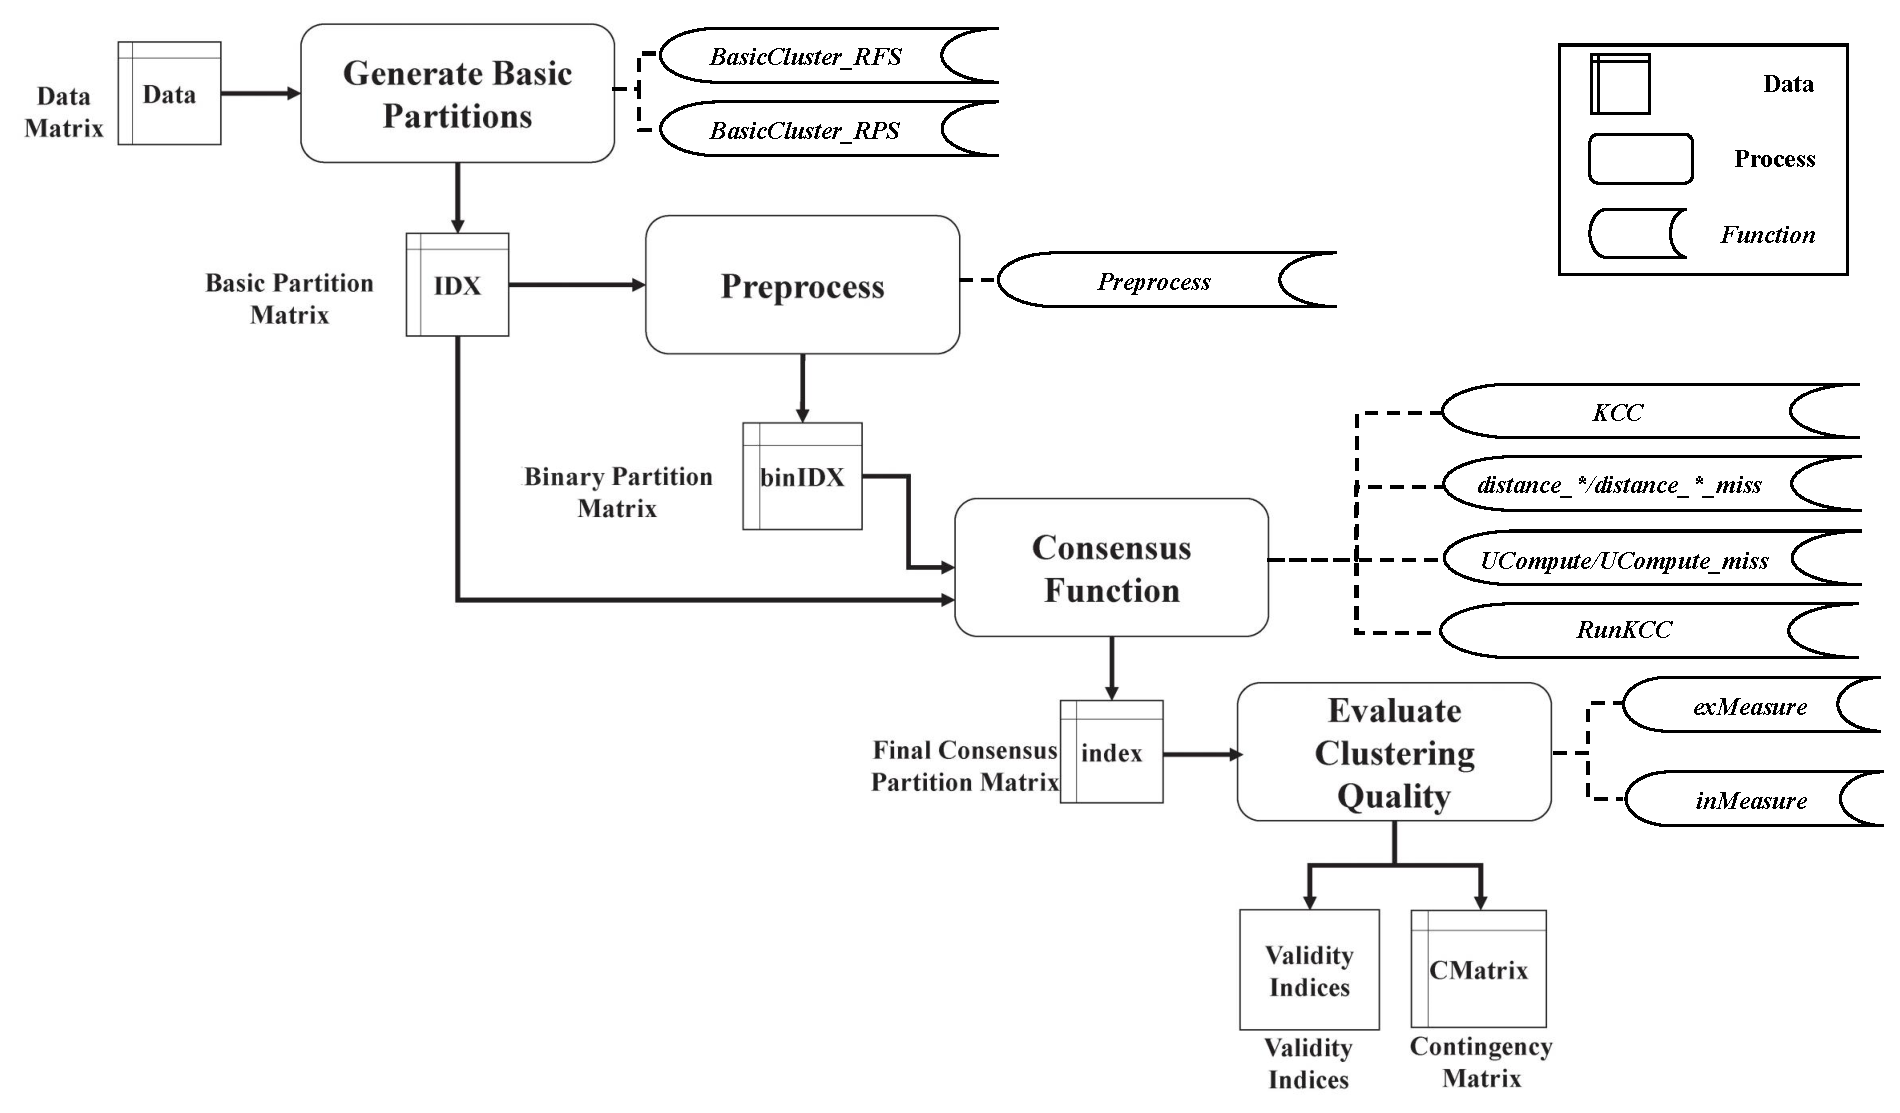
\includegraphics[width=0.85\textwidth]{fig/soft.eps}
\caption{Typical program flow of \KCC package.}\label{fig:soft} % \label should be placed after \caption
\end{figure*}

Figure~\ref{fig:soft} illustrates a typical program flow of using the \KCC package, which includes data preparation, basic partitions generation, consensus clustering preprocessing, consensus function, and clustering quality evaluation. We can see from Figure~\ref{fig:soft} that, in a typical flow for consensus clustering, a real-world matrix \textsf{Data} is first input to generate a basic partition matrix \textsf{IDX}. The basic partition matrix is then input to a \textsf{Preprocess} function to produce the sparse representation of $\mathcal{X}^{(b)}$, i.e., the binary matrix \textsf{binIDX}. The binary matrix \textsf{binIDX}, along with the basic partition matrix \textsf{IDX} is the input of the final consensus clustering via a $K$-means heuristic, also known as consensus function, which produces a consensus partition matrix \textsf{index}. Lastly, the clustering quality is evaluated with an \textsf{exMeasure} function, which outputs several external validity indices and a contingency matrix. We will take a detailed look at the important functions and fields in the Guides in Section~\ref{sec:guides}.

\section{Guides}\label{sec:guides}

\subsection{BasicCluster\_RFS}
This function generates basic partition results using $K$-means as a basic clustering algorithm with Random Feature Selection (RFS) strategy.

\syntax{IDX = BasicCluster\_RFS(Data, r, K, dist, nFeature)}

\begin{inputlist}
  \paramitem{Data}{input data matrix}
  \paramitem{r}{the predefined number of basic partitions in the cluster ensemble}
  \paramitem{K}{the predefined number of clusters in the basic partitions}
  \paramitem{dist}{the distance measure used in $K$-means clustering}
  \paramitem{nFeature}{the number of randomly selected partial features}
\end{inputlist}

\begin{outputlist}
  \paramitem{IDX}{a matrix indicating the cluster labels for data points in basic partitions}
\end{outputlist}

\begin{remark}
\noindent The parameter \texttt{Data} is an \textsf{n} $\times$ \textsf{p} matrix of data, whose rows correspond to \textsf{n} observations, and columns correspond to \textsf{p} features. The available options of the parameter \texttt{dist} can be found from the official documentation of the Matlab \textsf{kmeans} function, and the most widely used distance metric is \texttt{`sqEuclidean'}, which denotes the squared Euclidean distance. For \texttt{`sqEuclidean'}, the centroid for each cluster is calculated as the mean of the data points in that cluster. For selecting features, we first sample \textsf{nFeature} values uniformly at random without replacement from the integers \textsf{1} to \textsf{p}, where \textsf{p} is the dimension of all features in the input data. Then the sampled values are used as the indices of the selected features. The output \texttt{IDX} is a \textsf{n} $\times$ \textsf{r} cluster labels matrix for \textsf{n} data points in \textsf{r} basic partitions.
\end{remark}

\subsection{BasicCluster\_RPS}
This function generates basic partition results using $K$-means as a basic clustering algorithm with Random Parameter Selection (RPS) strategy.

\syntax{IDX = BasicCluster\_RPS(Data, r, K, dist, randKi)}

\begin{inputlist}
  \paramitem{Data}{input data matrix}
  \paramitem{r}{the predefined number of basic partitions in the cluster ensemble}
  \paramitem{K}{the groundtruth number of clusters for the input data}
  \paramitem{dist}{the distance measure used in $K$-means clustering}
  \paramitem{randKi}{the parameter regarding the number of clusters in the basic partitions}
\end{inputlist}

\begin{outputlist}
  \paramitem{IDX}{a \textsf{n} $\times$ \textsf{r} cluster labels matrix for \textsf{n} data points in \textsf{r} basic partitions}
\end{outputlist}

\begin{remark}
\noindent The parameter \texttt{K} indicates the groundtruth number of clusters for the input data, which is used as the lower bound of the randomized number of cluster for each basic partition when \texttt{randKi == 1}. The parameter \textsf{randKi} has the following options. If \texttt{randKi == 1}, this function generates a random number of cluster ranging from \texttt{K} to \texttt{sqrt(n)}, where $n$ is the number of input data instances; if \texttt{randKi} is set to a \textsf{r} $\times$ \textsf{1} vector, this function produces \textsf{r} basic partitions of which the $i$-th BP's number of clusters is \textsf{RandKi(i)}; otherwise, this function produces \textsf{r} basic partitions with each partition having equal number (i.e., \textsf{K}) of clusters.
\end{remark}

\subsection{Preprocess}
This function conduct some preprocessing on the input basic partition matrix \texttt{IDX} to produce the input for the final consensus clustering, as well as some auxiliary output variables that can help to save memory and accelerate computations.

\syntax{Ki, sumKi, binIDX, missFlag, missMatrix, distance, Pvector, weight = \\ Preprocess(IDX, U, n, r, w, utilFlag)}

\begin{inputlist}
  \paramitem{IDX}{the input basic partition matrix}
  \paramitem{U}{the parameter regarding the chosen utility function}
  \paramitem{n}{the number of data instances}
  \paramitem{r}{the number of basic partitions in the cluster ensemble}
  \paramitem{w}{the weight vector for all basic partitions}
  \paramitem{utiFlag}{whether to calculate utility function}
\end{inputlist}

\begin{outputlist}
  \paramitem{Ki}{a row vector indicating the number of clusters in all basic partitions}
  \paramitem{sumKi}{a matrix indicating the starting indexes for all basic partitions}
  \paramitem{binIDX}{a sparse representation of binarization of \textsf{IDX}}
  \paramitem{missFlag}{whether the input \textsf{IDX} matrix contains IBPs or not}
  \paramitem{missMatrix}{indices matrix of the non-zero entries in \textsf{IDX} if there exists IBPs}
  \paramitem{distance}{the distance function corresponding to a specific utility function}
  \paramitem{Pvector}{a row vector calculated from the contingency matrix}
  \paramitem{weight}{an adjusted weight vector adapted for convenient distance calculation}
\end{outputlist}

\begin{remark}
\noindent The parameter \textsf{U} is a \textsf{1} $\times$ \textsf{3} cell array. Its first cell \textsf{U\{1,1\}} defines the chosen type of the KCC utility function. It currently supports four different types of utility functions which correspond to four different $K$-means point-to-centroid distance functions, i.e., \textsf{`U\_c'} for Euclidean distance, \textsf{`U\_H'} for Kullback-Leibler Divergence, \textsf{`U\_cos'} for cosine similarity, and \textsf{`U\_Lp'} for Lp-norm. It is worth noting that \textsf{`U\_Lp'} corresponds the distance measure in $L_p$ spaces, which are function spaces defined using a natural generalization of the $p$-norm for finite-dimensional vector spaces. The second cell \textsf{U\{1,2\}} is a parameter specifying the chosen form of the KCC utility function, i.e., \textsf{`std'} for the Standard Form, and \textsf{`norm'} for the Normalized Form. The third cell \textsf{U\{1,3\}} is only required to be set when \textsf{`U\_Lp'} is chosen as the utility function. The settings of \textsf{p = 1}, \textsf{p = 2}, \textsf{p} $\rightarrow \infty$ correspond to the Manhattan distance, the euclidean distance and the chebyshev distance, respectively.  The parameter \texttt{w} is \textsf{r} $\times$ \textsf{1} weight vector, of which each entry indicates the weight value assigned to each basic partition in the optimization objective of consensus clustering. The parameter \texttt{utiFlag} is a variable indicating whether to calculate utility function during the iterative process of $K$-means clustering.

\noindent The output variable \textsf{missFlag} $\in \{0, 1\}$ indicates whether the input \textsf{IDX} matrix contains incomplete basic partitions (IBPs) or not. The output \textsf{missMatrix} is a mask matrix which represents the indices of the non-zero entries in \textsf{IDX} if there exists IBPs. The output variable \textsf{distance} determines the corresponding distance function to deal with the specific utility function defined by \textsf{U\{1,1\}}. The output vector \textsf{Pvector} is a \textsf{1} $\times$ \textsf{r} row vector calculated from the contingency matrix, i.e., $P^{(i)}_k$, which can later be used in calculating distance and utility functions. The output vector \textsf{weight} is a \textsf{r} $\times$ \textsf{1} adjusted weight vector adapted for convenient distance calculation in later $K$-means heuristic. 
\end{remark}

\subsection{KCC}
This function employs the $K$-means heuristic to generate a final consensus partition.

\syntax{sumbest, index, converge, utility = KCC(IDX, K, U, w, weight, distance, \\ maxIter, minThres, utilFlag, missFlag, missMatrix, n, r, Ki, sumKi, binIDX, Pvector)}

\begin{inputlist}
  \paramitem{IDX}{the input basic partition matrix}
  \paramitem{K}{the number of clusters in the consensus partition}
  \paramitem{U}{the parameter regarding the chosen utility function}
  \paramitem{w}{the weight vector for all basic partitions}
  \paramitem{weight}{an adjusted weight vector adapted for convenient distance calculation}
  \paramitem{distance}{the distance function corresponding to a specific utility function}
  \paramitem{maxIter}{the maximum number of iterations for the convergence}
  \paramitem{minThres}{the minimum reduced threshold of objective function}
  \paramitem{utiFlag}{whether to calculate utility function}
  \paramitem{missFlag}{whether there exist IBPs in \textsf{IDX}}
  \paramitem{missMatrix}{the indices matrix of the non-zero entries in \textsf{IDX} if there exists IBPs}
  \paramitem{n}{the number of data points}
  \paramitem{r}{the number of basic partitions in the cluster ensemble}
  \paramitem{Ki}{a row vector indicating the number of clusters in all basic partitions}
  \paramitem{sumKi}{a matrix indicating the starting indexes for all basic partitions}
  \paramitem{binIDX}{a sparse representation of binarization of \textsf{IDX}}
  \paramitem{Pvector}{a row vector calculated from the contingency matrix}
\end{inputlist}

\begin{outputlist}
  \paramitem{sumbest}{the optimal value of the consensus clustering's objective function}
  \paramitem{index}{the label vector for the final consensus partition}
  \paramitem{converge}{the iterative values of objective function}
  \paramitem{utility}{the final utility function value}
\end{outputlist}


\subsection{distance\_euc}
This function performs point-to-centroid distance calculation using euclidean distance measure.

\syntax{D = distance\_euc(U, C, weight, n, r, K, sumKi, binIDX)}

\begin{inputlist}
  \paramitem{U}{the \textsf{1} $\times$ \textsf{3} utility parameter cell array}
  \paramitem{C}{the centroid matrix}
  \paramitem{weight}{an \textsf{r} $\times$ \textsf{1} adjusted weight vector}
  \paramitem{n}{the number of data points}
  \paramitem{r}{the predefined number of basic partitions in the cluster ensemble}
  \paramitem{K}{the predefined number of clusters in the consensus partition}
  \paramitem{sumKi}{a matrix indicating the starting indexes for all basic partitions}
  \paramitem{binIDX}{a sparse representation of binarization of \textsf{IDX}}
\end{inputlist}

\begin{outputlist}
  \paramitem{D}{an \textsf{n} $\times$ \textsf{K} point-to-centroid distance matrix}
\end{outputlist}

\subsection{distance\_cos}
This function performs point-to-centroid distance calculation using cosine distance measure.

\syntax{D = distance\_cos(U, C, weight, n, r, K, sumKi, binIDX)}

\begin{inputlist}
  \paramitem{U}{the \textsf{1} $\times$ \textsf{3} utility parameter cell array}
  \paramitem{C}{the centroid matrix}
  \paramitem{weight}{an \textsf{r} $\times$ \textsf{1} adjusted weight vector}
  \paramitem{n}{the number of data points}
  \paramitem{r}{the predefined number of basic partitions in the cluster ensemble}
  \paramitem{K}{the predefined number of clusters in the consensus partition}
  \paramitem{sumKi}{a matrix indicating the starting indexes for all basic partitions}
  \paramitem{binIDX}{a sparse representation of binarization of \textsf{IDX}}
\end{inputlist}

\begin{outputlist}
  \paramitem{D}{an \textsf{n} $\times$ \textsf{K} point-to-centroid distance matrix}
\end{outputlist}


\subsection{distance\_kl}
This function performs point-to-centroid distance calculation using KL-divergence measure.

\syntax{D = distance\_kl(U, C, weight, n, r, K, sumKi, binIDX)}

\begin{inputlist}
  \paramitem{U}{the \textsf{1} $\times$ \textsf{3} utility parameter cell array}
  \paramitem{C}{the centroid matrix}
  \paramitem{weight}{an \textsf{r} $\times$ \textsf{1} adjusted weight vector}
  \paramitem{n}{the number of data points}
  \paramitem{r}{the predefined number of basic partitions in the cluster ensemble}
  \paramitem{K}{the predefined number of clusters in the consensus partition}
  \paramitem{sumKi}{a matrix indicating the starting indexes for all basic partitions}
  \paramitem{binIDX}{a sparse representation of binarization of \textsf{IDX}}
\end{inputlist}

\begin{outputlist}
  \paramitem{D}{an \textsf{n} $\times$ \textsf{K} point-to-centroid distance matrix}
\end{outputlist}


\subsection{distance\_lp}
This function performs point-to-centroid distance calculation using $L_p$ norm measure.

\syntax{D = distance\_lp(U, C, weight, n, r, K, sumKi, binIDX)}

\begin{inputlist}
  \paramitem{U}{the \textsf{1} $\times$ \textsf{3} utility parameter cell array}
  \paramitem{C}{the centroid matrix}
  \paramitem{weight}{an \textsf{r} $\times$ \textsf{1} adjusted weight vector}
  \paramitem{n}{the number of data points}
  \paramitem{r}{the predefined number of basic partitions in the cluster ensemble}
  \paramitem{K}{the predefined number of clusters in the consensus partition}
  \paramitem{sumKi}{a matrix indicating the starting indexes for all basic partitions}
  \paramitem{binIDX}{a sparse representation of binarization of \textsf{IDX}}
\end{inputlist}

\begin{outputlist}
  \paramitem{D}{an \textsf{n} $\times$ \textsf{K} point-to-centroid distance matrix}
\end{outputlist}


\subsection{distance\_euc\_miss}
This function performs point-to-centroid distance calculation over data with IBPs using euclidean distance measure.

\syntax{D = distance\_euc\_miss(U, C, weight, n, r, K, sumKi, binIDX, missMatrix)}

\begin{inputlist}
  \paramitem{U}{the \textsf{1} $\times$ \textsf{3} utility parameter cell array}
  \paramitem{C}{the centroid matrix}
  \paramitem{weight}{an \textsf{r} $\times$ \textsf{1} adjusted weight vector}
  \paramitem{n}{the number of data points}
  \paramitem{r}{the predefined number of basic partitions in the cluster ensemble}
  \paramitem{K}{the predefined number of clusters in the consensus partition}
  \paramitem{sumKi}{a matrix indicating the starting indexes for all basic partitions}
  \paramitem{binIDX}{a sparse representation of binarization of \textsf{IDX}}
  \paramitem{missMatrix}{the indices matrix of the non-zero entries in \textsf{IDX} if there exists IBPs}
\end{inputlist}

\begin{outputlist}
  \paramitem{D}{an \textsf{n} $\times$ \textsf{K} point-to-centroid distance matrix}
\end{outputlist}


\subsection{distance\_cos\_miss}
This function performs point-to-centroid distance calculation over data with IBPs using cosine distance measure.

\syntax{D = distance\_cos\_miss(U, C, weight, n, r, K, sumKi, binIDX, missMatrix)}

\begin{inputlist}
  \paramitem{U}{the \textsf{1} $\times$ \textsf{3} utility parameter cell array}
  \paramitem{C}{the centroid matrix}
  \paramitem{weight}{an \textsf{r} $\times$ \textsf{1} adjusted weight vector}
  \paramitem{n}{the number of data points}
  \paramitem{r}{the predefined number of basic partitions in the cluster ensemble}
  \paramitem{K}{the predefined number of clusters in the consensus partition}
  \paramitem{sumKi}{a matrix indicating the starting indexes for all basic partitions}
  \paramitem{binIDX}{a sparse representation of binarization of \textsf{IDX}}
  \paramitem{missMatrix}{the indices matrix of the non-zero entries in \textsf{IDX} if there exists IBPs}
\end{inputlist}

\begin{outputlist}
  \paramitem{D}{an \textsf{n} $\times$ \textsf{K} point-to-centroid distance matrix}
\end{outputlist}


\subsection{distance\_kl\_miss}
This function performs point-to-centroid distance calculation over data with IBPs using KL-divergence measure.

\syntax{D = distance\_kl\_miss(U, C, weight, n, r, K, sumKi, binIDX, missMatrix)}

\begin{inputlist}
  \paramitem{U}{the \textsf{1} $\times$ \textsf{3} utility parameter cell array}
  \paramitem{C}{the centroid matrix}
  \paramitem{weight}{an \textsf{r} $\times$ \textsf{1} adjusted weight vector}
  \paramitem{n}{the number of data points}
  \paramitem{r}{the predefined number of basic partitions in the cluster ensemble}
  \paramitem{K}{the predefined number of clusters in the consensus partition}
  \paramitem{sumKi}{a matrix indicating the starting indexes for all basic partitions}
  \paramitem{binIDX}{a sparse representation of binarization of \textsf{IDX}}
  \paramitem{missMatrix}{the indices matrix of the non-zero entries in \textsf{IDX} if there exists IBPs}
\end{inputlist}

\begin{outputlist}
  \paramitem{D}{an \textsf{n} $\times$ \textsf{K} point-to-centroid distance matrix}
\end{outputlist}


\subsection{distance\_lp\_miss}
This function performs point-to-centroid distance calculation over data with IBPs using $L_p$ norm measure.

\syntax{D = distance\_lp\_miss(U, C, weight, n, r, K, sumKi, binIDX, missMatrix)}

\begin{inputlist}
  \paramitem{U}{the \textsf{1} $\times$ \textsf{3} utility parameter cell array}
  \paramitem{C}{the centroid matrix}
  \paramitem{weight}{a \textsf{r} $\times$ \textsf{1} adjusted weight vector}
  \paramitem{n}{the number of data points}
  \paramitem{r}{the number of basic partitions in the cluster ensemble}
  \paramitem{K}{the predefined number of clusters}
  \paramitem{sumKi}{a matrix indicating the starting indexes for all basic partitions}
  \paramitem{binIDX}{the sparse representation matrix}
  \paramitem{missMatrix}{the indices matrix of the non-zero entries in \textsf{IDX} if there exists IBPs}
\end{inputlist}

\begin{outputlist}
  \paramitem{D}{an \textsf{n} $\times$ \textsf{K} point-to-centroid distance matrix}
\end{outputlist}


\subsection{UCompute}
This function performs utility calculation on data sets without missing values.

\syntax{util =  UCompute(index, U, w, C, n, r, K, sumKi, Pvector)}

\begin{inputlist}
  \paramitem{index}{an \textsf{n} $\times$ \textsf{1} cluster assignment matrix}
  \paramitem{U}{the \textsf{1} $\times$ \textsf{3} utility parameter cell array}
  \paramitem{w}{the \textsf{r} $\times$ \textsf{1} adjusted weight parameter vector}
  \paramitem{C}{the centroid matrix}
  \paramitem{n}{the number of data points}
  \paramitem{r}{the number of basic partitions in the cluster ensemble}
  \paramitem{K}{the predefined number of clusters in the consensus partition}
  \paramitem{sumKi}{a matrix indicating the starting indexes for all basic partitions}
  \paramitem{Pvector}{a \textsf{1} $\times$ \textsf{r} row vector calculated from the contingency matrix}
\end{inputlist}

\begin{outputlist}
  \paramitem{util}{the utility values calculated from the optimization objective of consensus clustering}
\end{outputlist}

\begin{remark}
\noindent The output \texttt{util} is a \textsf{2} $\times$ \textsf{1} cell array including a utility gain and an adjusted utility value.
\end{remark}


\subsection{UCompute\_miss}
This function performs utility calculation on data sets with missing values.

\syntax{util =  UCompute\_miss(index, U, w, C, n, r, K, sumKi, Pvector, M)}

\begin{inputlist}
  \paramitem{index}{an \textsf{n} $\times$ \textsf{1} cluster assignment matrix}
  \paramitem{U}{the \textsf{1} $\times$ \textsf{3} utility parameter cell array}
  \paramitem{w}{the \textsf{r} $\times$ \textsf{1} adjusted weight parameter vector}
  \paramitem{C}{the centroid matrix}
  \paramitem{n}{the number of data points}
  \paramitem{r}{the number of basic partitions in the cluster ensemble}
  \paramitem{K}{the predefined number of clusters in the consensus partition}
  \paramitem{sumKi}{a matrix indicating the starting indexes for all basic partitions}
  \paramitem{Pvector}{a \textsf{1} $\times$ \textsf{r} row vector calculated from the contingency matrix}
  \paramitem{M}{a mask matrix indicating the indices of the non-zero entries in \textsf{IDX}}
\end{inputlist}

\begin{outputlist}
  \paramitem{util}{the utility values calculated from the optimization objective of consensus clustering}
\end{outputlist}


\subsection{RunKCC}
This function combines the two functions, i.e., \textsf{Preprocess} and \textsf{KCC}, for finding the consensus partition in one step.

\syntax{[pi\_sumbest, pi\_index, pi\_converge, pi\_utility, t] = RunKCC(IDX, K, U, w, rep, maxIter, minThres, utilFlag)}

\begin{inputlist}
  \paramitem{IDX}{the basic partition matrix}
  \paramitem{K}{the predefined number of clusters in the consensus partition}
  \paramitem{U}{the \textsf{1} $\times$ \textsf{3} utility parameter cell array}
  \paramitem{w}{the \textsf{r} $\times$ \textsf{1} adjusted weight parameter vector}
  \paramitem{rep}{the number of repeated KCC experiments for selecting the best result}
  \paramitem{maxIter}{the maximum number of iterations for the convergence}
  \paramitem{minThres}{the minimum reduced threshold of objective function}
  \paramitem{utiFlag}{whether to calculate utility function}
\end{inputlist}

\begin{outputlist}
  \paramitem{pi\_sumbest}{the value of objective function for the best KCC experiment}
  \paramitem{pi\_index}{the cluster assignment matrix in the consensus partition for the best KCC experiment}
  \paramitem{pi\_converge}{the iterative values of objective function for the best KCC experiment}
  \paramitem{pi\_utility}{the utility values for the best KCC experiment}
  \paramitem{t}{the execution time cost of the whole process for this function}
\end{outputlist}

\subsection{exMeasure}
This function assesses the clustering quality of the results obtained by a clustering algorithm.

\syntax{[Acc, Rn, NMI, VIn, VDn, labelnum, ncluster, cmatrix] = exMeasure(cluster, true\_label)}

\begin{inputlist}
  \paramitem{cluster}{a \textsf{n} $\times$ \textsf{1} cluster assignment matrix returned by a clustering algorithm}
  \paramitem{true\_label}{the true class labels for the data points}
\end{inputlist}

\begin{outputlist}
  \paramitem{Acc}{the classification accuracy}
  \paramitem{Rn}{the normalized Rand statistic}
  \paramitem{NMI}{the normalized mutual information}
  \paramitem{VIn}{the normalized Variation of Information}
  \paramitem{VDn}{the normalized van Dongen criterion}
  \paramitem{labelnum}{the number of unique labels in the groundtruth data}
  \paramitem{ncluster}{the number of clusters returned by the algorithm}
  \paramitem{cmatrix}{a \textsf{ncluster} $\times$ \textsf{labelnum} contingency matrix}
\end{outputlist}

\begin{remark}
\noindent This function implements five external validity indices, including classification accuracy~\cite{nguyen2007consensus} ($CA$), the normalized mutual information~\cite{cover2012elements} ($NMI$), the normalized Rand statistic~\cite{rand1971objective} ($R_n$), the normalized van Dongen criterion~\cite{dongen2000performance} ($VD_n$), and the normalized Variation of Information~\cite{cover2012elements} ($VI_n$). In implementing the \textsf{exMeasure} function, we utilize a function called \textsf{bestMap} written by \cite{CHH05}, in which the Hungarian method~\cite{carpaneto1980algorithm} is employed to resolve the label assignment issue in clustering.
\end{remark}

% References
\begin{small}
\bibliography{references}
\bibliographystyle{ACM-Reference-Format}
\end{small}

\end{document}
